\documentclass[hyperref={pdfpagelabels=false},t,10pt]{beamer}
\usepackage[utf8]{inputenc}
\usepackage[english]{babel}
\usepackage[T1]{fontenc}
\usepackage[default,scale=.95]{opensans}
\usepackage[most]{tcolorbox}
\usepackage{amsmath,amssymb}
\usepackage{xcolor}

%\usepackage{enumitem}



\usetheme[cd2018]{tud}
\setbeamercolor{normal text}{fg=black}
\colorlet{alert}{cdblue}
\setbeamercolor{alerted text}{fg=cdblue}
\setbeamerfont{frametitle}{size=\Large,family=\sffamily,series=\sbseries}


\DeclareRobustCommand\sbseries{\fontseries{sb}\selectfont}
\DeclareTextFontCommand{\textsb}{\sbseries}


\title{TITLE}
\author[© author]{Maik Thanh Nguyen}
\institute{Technische Universit\"at Dresden}
\datecity{CONFERENCE}
\date{DATE}

%\newtheorem{theorem}{Theorem}
%\newtheorem{definition}{Definition}

\begin{document}

%%%% Uncomment the following line to set background image to main slide
%%%% (parameter sets transparency)
%\setbeamertemplate{tud background}[image/shaded]{background.jpg}{0.5}
\addtocounter{framenumber}{-1}
\maketitle

\begin{frame}
  \frametitle{Content}

  \begin{itemize}
  \item Syntax and semantics
    \begin{itemize}
        \item Kripke frames
        \item Topological space
        \item Neighbourhood frames
     \end{itemize}
  \item Multimodal logic and product of frames/spaces and logics
    \begin{itemize}
      \item Multimodal logic and product of frames
      \item Horizontal and Vertical topology/functions
      \item Product of logics and the logic T
    \end{itemize}
  \item Main result and ideas
  \end{itemize}
\end{frame}

\begin{frame}
  \frametitle{Basic modal language, Kripke frames and models}
  \begin{itemize}
    \item Basic modal langauge extends classical propositional logic. Formally:
  \end{itemize}
    
    \begin{definition}
      Let Prop be a set of variable. Then a formula $\phi$ is defined as follows:
          $$\phi ::= p \mid \bot \mid \neg \phi \mid \phi \lor \phi \mid \textcolor{red}{\Box \phi}$$
           where $\Box$ is a modal operator and $p \in$ Prop  
    \end{definition}
    %Other connectives are expressed through $\neg$ and $\lor$ and dual modal operator $\lozenge$ as $\lozenge \phi = \neg \Box \neg \phi$. 
     \pause

    \begin{definition}
    A frame $F = (W,R)$ is a pair where   
    \begin{itemize}
      \item $W$ is a non-empty set of worlds
      \item $R \subseteq W \times W $ is a binary relation
    \end{itemize}

    A model is a pair $M = (F,R)$ where $V$ is a valuation and is of the form $V : Prop \rightarrow 2^W$


    \end{definition}

\end{frame}

\begin{frame}
  \frametitle{Example}
  \begin{itemize}
    \item Let $\phi = \Box p$ and $M = (W,R,V)$ with $W = \{w_1,w_2,w_3,w_4,w_5\}$, $V(p) = \{w_3,w_4,w_5\}$ and $R = $
  \end{itemize}
  \centering
  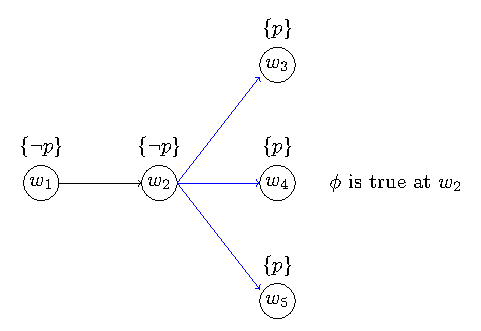
\includegraphics[width=0.55\textwidth]{Example1.pdf}
\end{frame}



\begin{frame}
  \frametitle{Kripke semantics}

  \begin{definition}
      Let $M = (F,V)$ be a model and $w \in W$ a state in $M$. A formula being true at $w$ is inductively defined as: 
      \begin{align*}
        M, w &\Vdash p &&\text{ iff } w \in V(p) \\
        M, w &\Vdash \bot  &&\text{ never } \\
        M, w &\Vdash \neg \phi &&\text{ iff not } M, w \Vdash \phi \\ 
        M, w &\Vdash \phi \lor \psi &&\text{ iff } M,w \Vdash \phi \lor M,w \Vdash \psi \\
        M, w &\Vdash \textcolor{red}{\Box \phi} &&\text{ iff } \forall v \in W : wRv \rightarrow M, v \Vdash \phi \\
        M, w &\Vdash \textcolor{red}{\lozenge \phi} &&\text{ iff } \exists v \in W : wRv \land M,v \Vdash \phi
    \end{align*}  
  \end{definition}


  
\end{frame}



\begin{frame}
  \frametitle{Topological space}
  \begin{itemize}
    \item Topological space deals with open sets, it can describes which points are "nearby" \pause %truth is defined differently 
    \begin{definition}
             A topological space is a pair $(X, \tau)$, where $\tau$ (called topology) is a collection of subsets of $X$ (open sets) such that: \pause
        \begin{itemize}
          \item $\emptyset$ and $X$ are open
          \item the union of arbitrary collection of open sets is open
          \item the intersection of finite collection of open sets is open
        \end{itemize} \pause
          A topological model is a structure $M = (X,\tau, \upsilon)$ where $(X, \tau)$ is a topological space and $\upsilon$ a valuation of the form $\upsilon : Prop \rightarrow 2^X$  
    \end{definition}
    \end{itemize}
    \end{frame}

  \begin{frame}
  
    \frametitle{Example}
    \begin{itemize}
      \item  Let $(X,\tau)$ be a topological space with 
      $X = \{1,2,3\}$, $\tau = \{\emptyset, \{1\}, \{2\}, \{1,2\}, W\}$ and $V(p) = \{1,2\}$. Furthermore, let $\phi = \Box p$.
      \pause
    \end{itemize}
    \centering
    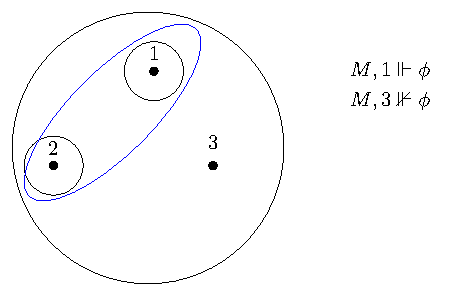
\includegraphics[width=0.55\textwidth]{Example2.pdf}

  \end{frame}


\begin{frame}
  \frametitle{Topological semantics}
  Let $M = (X, \tau, \upsilon)$ be a topological model and $x \in X$ a point in $M$. A formula being true at $x$ is inductively defined as:

  \[
\begin{aligned}
    M, x &\vDash p &&\text{iff } x \in v(p) \\
    M, x &\vDash \bot &&\text{never} \\
    M, x &\vDash \neg \phi &&\text{iff } M, x \nvDash \phi \\
    M, x &\vDash \phi \lor \psi &&\text{iff } M, x \vDash \phi \text{ or } M, x \vDash \psi \\
    M, x &\vDash \textcolor{red}{\Box \phi} &&\text{iff }\exists U \in \tau \text{ such that } x \in U \text{ and } \forall u \in U,\; M, u \vDash \phi \\
    M, x &\vDash \textcolor{red}{\lozenge \phi} &&\text{iff }\forall U \in \tau: \text{if }x \in U \rightarrow \exists u \in U,\; M, u \vDash \phi
\end{aligned}
\]

\end{frame}




\begin{frame}
  \frametitle{Neighbourhood frames}
    \begin{itemize}
      \item generalize Kripke semantics
      \item captures non-normal modal logics
    \end{itemize}

    \pause
    \begin{definition}
      A neighbourhood frame is a pair $(X, \tau)$ where $\tau$ is a function $\tau : X \rightarrow 2^{2^X}$. \newline
      A neighbourhood model is a structure $M = (X, \tau, \upsilon)$, where $\upsilon$ is a valuation of the form $\upsilon : Prop \rightarrow 2^X$
    \end{definition}
\end{frame}

\begin{frame}
  \frametitle{Example}
      Assume $\phi = \Box p$. Let $W = \{1,2,3\}$, $V(p) = \{1,2\}$ and 
    \[
            \tau(x) = 
            \begin{cases}
                1 \rightarrow \{\{1\}, \{3\}, W\} \\
                2 \rightarrow \{\{2\}, \{1,2\}, W\} \\
                3 \rightarrow \{\{3\}, \{1,3\}\}
            \end{cases}
    \] 
    \centering
      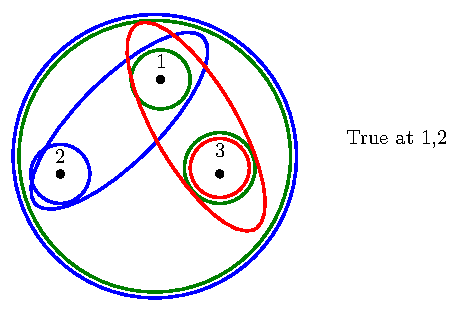
\includegraphics[width=0.55\textwidth]{Example3.pdf}
\end{frame}

\begin{frame}
  \frametitle{Neighbourhood semantics}
  Let $M = (X,\tau,\upsilon)$ be a neighbourhood model and $x \in X$ a point in $M$. A formula being true at x is inductively defined as:
      \begin{align*}
        M,x &\Vdash p &&\text{iff } x \in V(p)\\
        M,x &\Vdash \bot &&\text{never } \\
        M,x &\Vdash \neg \phi &&\text{iff } M,x \nVdash \phi\\
        M,x &\Vdash \phi \lor \psi &&\text{iff } M,x \vDash \phi \lor M,x \vDash \psi\\
        M,x &\Vdash \textcolor{red}{\Box \phi} &&\text{iff } \exists V \in \tau(x) \forall y \in V : M,y \models \phi
    \end{align*}

\end{frame}


\begin{frame}
  \frametitle{Modal logic and the logic $T$}
  \begin{definition}
    A modal logic is a set of modal formulas containing all propositional tautologies, closed under Substitution ($\frac{\phi(p_i)}{\phi(\psi)}$), Modus Ponens $(\frac{\phi, \phi \rightarrow \psi}{\psi})$. \newline \newline \pause
    A modal logic is normal, if it contains $\Box (p \rightarrow q) \rightarrow (\Box p \rightarrow \Box q)$ (K) and is closed under Generalization $(\frac{\phi}{\Box \phi})$
  \end{definition}

  \begin{definition}
      $T = K + \Box p \rightarrow p$
  \end{definition}
\end{frame}



\begin{frame}
  \frametitle{Multimodal logic and product of frames}
  \begin{itemize}
    \item Mutlimodal logic allows us to reason about knowledge,time etc. simultaneously 
    \item for example we can combine temporal and epistemic logic to reason about "when does the agent knows something" \pause % consider the product of frames to interpret the formulas 
    \item horizontal and vertical relation allows us to reason in one dimension \pause% , for example we a fix time point and ask what does the agent knows at that time?
    \begin{definition}
      Let $F = (W, R_1)$ and $G = (V, R_2)$. We define the Kripke product on $W \times V$ as : 
        \begin{align*}
              (w,v)R_1'(w',v') &\text{ iff } wR_1w' \mbox{ and } v = v' \text{  (horizontal)} \\
              (w,v)R_2  '(w',v') &\text{ iff } w = w' \mbox{ and } vR_2v' \text{(vertical)}
      \end{align*}  
    \end{definition}




    %\item Let $L_1$ and $L_2$ be two modal logics with one modality $\Box$. Then the fusion
    %is defined as: $$L_1 \otimes L_2 = K_2 + L_{1 \Box \rightarrow \Box_1} + L_{2 \Box \rightarrow \Box_2}$$
   % \item we consider the product of frames to evaluate multimodal formulas
  \end{itemize}
\end{frame}

\begin{frame}
  \frametitle{Example and Fusion of logics} %It’s also possible to combine modal logics with fusion
    %\centering

    \begin{tikzpicture}
       \node[draw, circle, inner sep=1.5pt] (A) at (0,0) {\small 3};
       \node[draw, circle, inner sep=1.5pt] (B) at (0,-1) {$2$};
       \node[draw, circle, inner sep=1.5pt] (C) at (0,-2) {$1$};
       \node at (-0.5,0.5) {$R_1$};

       \draw [blue,->] (C) -- (B);
       \draw [blue, ->] (B) -- (A);

       \node[draw, circle, inner sep=1.5pt] (D) at (4,-1) {$a$};
       \node[draw, circle, inner sep=1.5pt] (E) at (5,-1) {$b$};

       \draw [red, ->] (D) -- (E);
    \end{tikzpicture}
\pause

    
    \begin{definition}
      Let $L_1$ and $L_2$ be modal logics with one modality $\Box$. The fusion is defined as:
      $$ L_1 \otimes L_2 = K_2 + L_{1(\Box \rightarrow \Box_1)} L_{2(\Box \rightarrow \Box_2)} $$    
    \end{definition}



\end{frame}

\begin{frame}
  \frametitle{Horizontal and Vertical topology}
  \begin{itemize}
    \item in topological space, horizontal and vertical can be also defined \pause
  \end{itemize}
  Let \( \mathcal{X} = (X, \chi) \) and \( \mathcal{Y} = (Y, \upsilon) \) be topological spaces and \( N \subseteq X \times Y \) \newline

\begin{description}
  \item[Horizontally open:] \(N\) is horizontally open iff 
  \[
    \forall (x, y) \in N\; \exists U \in \chi \text{ such that } x \in U \text{ and } U \times \{y\} \subseteq N.
  \]

  \item[Vertically open:] \(N\) is vertically open iff 
  \[
    \forall (x, y) \in N\; \exists V \in \upsilon \text{ such that } y \in V \text{ and } \{x\} \times V \subseteq N.
  \]

\end{description}
\begin{itemize}
  \item $\tau_1$ (horizontal topology) is the set of all horizontally open sets and $\tau_2$ (vertical topology) the set of all vertically open sets.
\end{itemize}



\end{frame}

\begin{frame}
  \frametitle{Illustration, standard product}
    \centering
    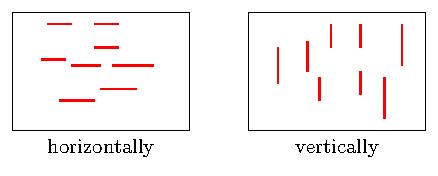
\includegraphics[width=0.55\textwidth]{Example4.pdf} \pause
  \begin{itemize}
    \item we can also reason in both directions at once with the standard topology
    \item we denote the standard toplogy as $\tau$ where 
    $$\tau = \{N \subseteq X \times Y \mid \exists U \in \chi \exists V \in \upsilon: N = U \times V\}$$  
  \end{itemize}

\end{frame}

\begin{frame}
  \frametitle{horizontal, vertical and standard functions}
  Let $\mathcal{X}$ = ($X$, $\tau_1$) and $\mathcal{Y}$ = ($Y$, $\tau_2$) be two n-frames. We define the full product as
    $$\mathcal{X} \times_n^+  \mathcal{Y} = (X \times Y, \tau_1', \tau_2', \tau) \text{ where}$$
    $$ \tau_1'(x,y) = \{ U \subseteq \mbox{X} \times \mbox{Y} \mid \exists V \in \tau_1(x) : V \times  \{ y \} \subseteq U \}$$
    $$ \tau_2'(x,y) = \{ U \subseteq \mbox{X} \times \mbox{Y} \mid \exists V \in \tau_2(y) : \{ x \} \times V \subseteq U \}$$
        $$ \tau(x,y) = \{ U \subseteq \mbox{X} \times \mbox{Y} \mid \exists W \in \tau_1(x) \, \exists V \in \tau_2(y) : W \times V \subseteq U \}$$   
\end{frame}

\begin{frame}
  \frametitle{Product of logics and the logic T}
  Let $L_1$ and $L_2$ be two unimodal logic. We define the full n-product of them as:
  $$L_1 \times_n^+ L_2 =  Log(\{\mathcal{X} \times_n^+ \mathcal{Y} \mid \mathcal{X} \Vdash L_1 \text{ and } \mathcal{Y} \Vdash L_2 \})$$ \pause
  \begin{itemize}
    \item this thesis deals with the logic $T$
    \item $T = K + \Box p \rightarrow p$
  \end{itemize}
\end{frame}

\begin{frame}
  \frametitle{Main Research Question}
  \begin{itemize}
    \item Does the following equality holds? 
    $$T \otimes T \otimes T + \Box p \rightarrow \Box_1 p \land \Box_2 p = T \times_n^+ T$$
    where $T \otimes T \otimes T = K_3 + T_{\Box} + T_{(\Box \rightarrow \Box_1)} + T_{(\Box \rightarrow \Box_2)}$ is the logic with three modalities 
    and $\Box p \rightarrow \Box_1 p \land \Box_2 p$ the interaction axiom \pause
    \item main motivation comes from epistemic logic 
    \item we will only sketch the right to left inclusion
    \item proof is splitted into two parts (ideas are from [1], [2])
  \end{itemize}
\end{frame}

\begin{frame}
  \frametitle{Sketch of the main ideas}
  \begin{itemize}
    \item Pick $\mathcal{C} = \{F \mid F \Vdash T \otimes T\otimes T + \Box p \rightarrow \Box_1 p \land \Box_2 p\}$  \pause
    \item Show $Log(\mathcal{C}) = T \otimes T \otimes T + \Box p \rightarrow \Box_1 p \land \Box_2 p$ via Sahlqvist Theorem
    \item We show finite model property of the logic with Filtration Theorem \pause
    \item Construct an infinite branching and infinite depth tree with three reflexive relations ($T_{\omega,\omega,\omega[rn]}$) \pause
    \item Show $Log(T_{\omega,\omega,\omega[rn]}) = T \otimes T \otimes T+ \Box p \rightarrow \Box_1 p \land \Box_2 p$
    \item By FMP pick a finite frame $F \in \mathcal{C}$ and construct a bounded morphism from $T_{\omega,\omega,\omega[rn]}$ to $F$
  \end{itemize}

\end{frame}

\begin{frame}
  \frametitle{Sketch continue}
  $$Log(T_{\omega,\omega,\omega[rn]}) = T \otimes T \otimes T+ \Box p \rightarrow \Box_1 p \land \Box_2 p$$
  \begin{itemize}
    \item we introduce a simpler version of $T_{\omega,\omega,\omega[rn]}$ which is $T_{\omega[rn]}$ \pause
    \item construct a neighbourhood version of $T_{\omega[rn]}$ called $N_\omega(T_{\omega[rn]})$ 
    \item we can show $T = Log(N_\omega(T_{\omega[rn]}))$ \pause
    \item construct a bounded morphism $$N_\omega(T_{\omega[rn]}) \times_n^+ N_\omega(T_{\omega[rn]}) \rightarrow T_{\omega,\omega,\omega[rn]}$$
    \item with some further steps we can conclude $$T \times_n^+ T \subseteq T \otimes T \otimes T + \Box p \rightarrow \Box_1 p \land \Box_2 p$$
  \end{itemize}

\end{frame}  

\begin{frame}
  \frametitle{$T_{\omega,\omega,\omega[rn]}$ and a more detailed sketch}
  %\centering
  %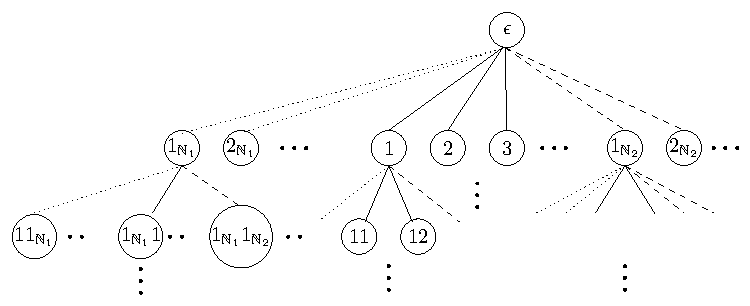
\includegraphics[width=0.73\textwidth]{Example7.pdf} \newline\pause
  %\begin{tcolorbox}[colback=blue!5!white, colframe=blue!75!black, title=Bounded morphism, fontupper=\sffamily\small]
 %     Let $F = (W,R_1,R_2,...)$ and $F' = (W',R_1',R_2',...)$ be two frames. A bounded morphism is a function $f: W \rightarrow W'$ with the following conditions:
   %   $$\text{If } uR_iv \text{ then } f(u)R_i'f(v)$$
  %    $$\text{If } f(w)R_i'v' \text{ then } \exists v\in W: wRv \text{ and } f(v) = v'$$
 % \end{tcolorbox}
    Let $F = (W,R_1,R_2,...)$ and $F' = (W',R_1',R_2',...)$ be two frames. A bounded morphism $f: W \rightarrow W'$ can be illustrated as:
    \centering
    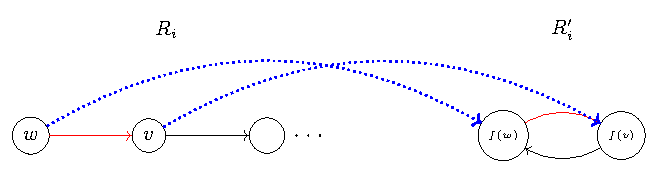
\includegraphics[width=0.73\textwidth]{Example8.pdf}

    \vspace{1cm}
    \begin{tikzpicture}
      \node[draw, circle, minimum size=0.2cm] (A) at (0,0) {$w$};
      \node[draw, circle, minimum size=0.2cm] (B) at (0,-1.5) {$v$};
      \node[draw, circle, font=\tiny\itshape] (C) at (1.8,0) {$f(w)$};
      \node[draw, circle, font=\tiny\itshape] (D) at (1.8,-1.5){$f(v)$};
      

      \draw [->] (C) -- (D);
      \draw[->, bend left=30,dotted, thick] (A) to (C); \pause
      \draw [->,red] (A) -- (B);
      \draw [->, bend left=330,dotted, thick,red] (B) to (D);
    \end{tikzpicture}

\end{frame}

\begin{frame}
  \frametitle{$T_{\omega,\omega,\omega[rn]}$ and a more detailed sketch}
  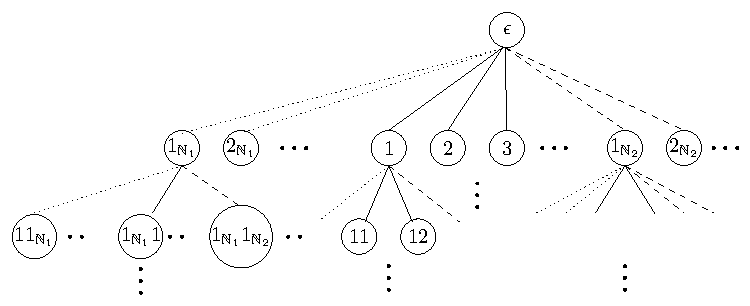
\includegraphics[width=0.73\textwidth]{Example7.pdf} \newline\pause

  \begin{tikzpicture}[yshift=-0.15cm]
    \node[draw, circle, minimum size=0.2cm] (A) at (0,0) {$x$};
    \node[draw, circle, minimum size=0.2cm] (B) at (1,1) {$y$};
    \node[draw, circle, minimum size=0.2cm] (C) at (1,-1) {$z$};
    \draw [->] (A) to (B);
    \draw [->] (A) to (C);

    \node at (-0.5,1.5) {$R_1'$};

    \node[draw, circle, minimum size=0.2cm] (D) at (4,0) {$x$};
    \node[draw, circle, minimum size=0.2cm] (E) at (5,1) {$y$};
    \node[draw, circle, minimum size=0.2cm] (F) at (5,-1) {$z$};
    \draw [->] (D) to (E);
    \draw [->] (E) to (F);

    \node at (3.5,1.5) {$R_2'$};

    \node[draw, circle, minimum size=0.2cm] (G) at (7.5,0) {$x$};
    \node[draw, circle, minimum size=0.2cm] (H) at (9,1) {$y$};
    \node[draw, circle, minimum size=0.2cm] (I) at (9,-1) {$z$};

    \draw [->] (G) to (H);
    \draw [->] (G) to (I);

    \draw[->,  bend left=30, thick] (H) to (I);
    \draw[->, bend left=30,thick] (I) to (H);

    \node at (7.5,1.5) {$R'$};
    \pause



  \end{tikzpicture}
\end{frame}


\begin{frame}
  \frametitle{Future works}
  \begin{itemize}
    \item Many ways to continue the research
    \item Discover how it works for logic $K$
    \item Combine different logics for example $D \times_n^+ K, T \times_n^+ K, ...$
    \item For logic $\Lambda$ with $T \subseteq \Lambda \subseteq S4$, does the following hold:
     $$\Lambda \otimes \Lambda \otimes \Lambda + \Box p \rightarrow \Box_1 p \land \Box_2 p = \Lambda \times_n^+ \Lambda$$
  
  \end{itemize}
\end{frame}

\begin{frame}
  \vspace{3.5cm}
  \centering
  \begin{tikzpicture}
    \node[font=\Large] at (0,0) {Conclusion};
  \end{tikzpicture}
\end{frame}

\begin{frame}
  \frametitle{References}
    [1] Johan van Benthem, Guram Bezhanishvili, Balder ten Cate, and Darko Sarenac.\\
    Multimodal logics of products of topologies. \textit{Studia Logica}, 84:369–392, 2006. \newline

    [2] Andrei Kudinov. Modal logic of some products of neighbourhood frames.\\
    In \textit{Advances in Modal Logic, Volume 9}, pages 286–294, London, 2012. College Publications.
\end{frame}


\end{document}
